\documentclass[a4paper, 12pt, oneside]{book}

%% подключаем стандарт библиографии
\bibliographystyle{gost71u} 

%% for envirovemt "abstract" in class book
\newenvironment{abstract}{}{}
\usepackage{abstract}

%% подключаем преамбулу, в ней содержатся подключение всех необходимых пакетов
%%% Работа с русским языком
\usepackage{cmap}			 % поиск в PDF
\usepackage{mathtext} 		 % русские буквы в формулах
\usepackage[T2A]{fontenc}	 % кодировка
\usepackage[utf8]{inputenc}	 % кодировка исходного текста
\usepackage[russian]{babel}	 % локализация и переносы

%%% Пакеты для работы с математикой
\usepackage{amsmath,amsfonts,amssymb,amsthm,mathtools}
\usepackage{icomma}

%% Номера формул
\mathtoolsset{showonlyrefs=true} % Показывать номера только у тех формул, на которые есть \eqref{} в тексте.
\usepackage{leqno}               % Немуреация формул слева

%% Шрифты
\usepackage{euscript}	 % Шрифт Евклид
\usepackage{mathrsfs}    % Красивый матшрифт

%% Поля (геометрия страницы)
\usepackage[left=3cm,right=2cm,top=2cm,bottom=2cm,bindingoffset=0cm]{geometry}

%% Русские списки
\usepackage{enumitem}
\makeatletter
\AddEnumerateCounter{\asbuk}{\russian@alph}{щ}
\makeatother

%%% Работа с картинками
\usepackage{caption}
\captionsetup{justification=centering} % центрирование подписей к картинкам
\usepackage{graphicx}                  % Для вставки рисунков
\usepackage{transparent}               % Настройка прозрачности
\graphicspath{{images/}{images2/}}     % папки с картинками
\setlength\fboxsep{3pt}                % Отступ рамки \fbox{} от рисунка
\setlength\fboxrule{1pt}               % Толщина линий рамки \fbox{}
\usepackage{wrapfig}                   % Обтекание рисунков и таблиц текстом


%%% Работа с таблицами
\usepackage{array,tabularx,tabulary,booktabs} % Дополнительная работа с таблицами
\usepackage{longtable}                        % Длинные таблицы
\usepackage{multirow}                         % Слияние строк в таблице

%% Красная строка
\setlength{\parindent}{2em}
\usepackage{indentfirst}

%% Интервалы
\linespread{1}
\usepackage{multirow}

%% Верхний колонтитул
\usepackage{fancyhdr}
\pagestyle{fancy}

%% TikZ
\usepackage{tikz}
\usetikzlibrary{graphs,graphs.standard}

%% Перенос знаков в формулах (по Львовскому)
\newcommand*{\hm}[1]{#1\nobreak\discretionary{}{\hbox{$\mathsurround=0pt #1$}}{}}

%% дополнения
\usepackage{float}   % Добавляет возможность работы с командой [H] которая улучшает расположение на странице
\usepackage{gensymb} % Красивые градусы
\usepackage{caption} % Пакет для подписей к рисункам, в частности, для работы caption*

% подключаем hyperref (для ссылок внутри  pdf)
\usepackage[unicode, pdftex]{hyperref}


\begin{document}
    \setlength{\headheight}{16pt}
    %% титульник
    \begin{center}
    %% *название института*
    \large\textbf{МИНИСТЕРСТВО ОБРАЗОВАНИЯ И НАУКИ РОССИЙСКОЙ ФЕДЕРАЦИИ \\
    МОСКОВСКИЙ ФИЗИКО-ТЕХНИЧЕСКИЙ ИНСТИТУТ \\
    (ГОСУДАРСТВЕННЫЙ УНИВЕРСИТЕТ, НАУЧНО-ИССЛЕДОВАТЕЛЬСКИЙ ИНСТИТУТ)} \\
    \vspace{1cm}

    %% *факультет/физтех-школа*
    Физтех-школа Аэрокосмических Технологий \\

    %% *название базовой кафедры и лаборатории*
    %% в случае ненадобности можно удалить
    Кафедра космического приборостроения \\

    \vspace{3em}

    Выпускная квалификационная работа бакалавра
\end{center}

\begin{center}
    \vspace{\fill}
    %% *название вашей работы*
    \LARGE{Разработка алгоритмов автоматического контроля и анализа качества синтеза радиолокационного изображения}

    \vspace{\fill}
\end{center}


\begin{flushright}
    \vspace{4em}
    \textbf{Автор:} \\
    Студент 4-го курса \\
    Рязанов Данила Сергеевич \\
    \vspace{2em}
    \textbf{Научный руководитель:} \\
    кандидат технических наук \\
    Мордвинов Александр Евгеньевич \\

\end{flushright}

\vspace{7em}

\begin{center}
    %% *лого*
    
\includegraphics[width=100 pt]{MIPT_logo.jpg}\\
    Москва \the\year{}
\end{center}

% выключаем отображение номера для этой страницы (титульник)
\thispagestyle{empty}

%\newpage
\setcounter{page}{2}
\fancyfoot[c]{\thepage}
%% *надпись над верхним колонтинулом*
%% в случае ненадобности можно удалить


    \setcounter{page}{0}
    %% аннотоция
    %\begin{abstract}

    \begin{center}
        \large{Разработка алгоритмов автоматического контроля и анализа качества синтеза радиолокационного изображения} \\
    \large\textit{Рязанов Данила Сергеевич} \\[1 cm]

	Задачей данной работы является разработка алгоритмов для автоматического контроля качества синтеза радиолокационного изображения. 

    \vfill

    \textbf{Abstract} \\[1 cm]

    \end{center}

\end{abstract}
\newpage

    %содержание
    \tableofcontents{}
    %\newpage

    \chapter{Введение}
\label{sec:Chapter0} \index{Chapter0}

\section{Вступление}

	В настоящее время радиолокаторы с синтезированной апертурой (РСА) используются для решения различных задач по мониторингу поверхности Земли. В отличие от оптической съемки, РСА обеспечивает всепогодное круглосуточное наблюдение за земной поверхностью [1]. В процессе работы радиолокатора выполняется периодическое излучение зондирующего импульса. В интервалах между стробами излучения выполняется запись отраженного от поверхности Земли сигнала, на основе которого формируется радиоголограмма [1]. При помощи алгоритмов синтеза из записанной радиоголограммы формируется радиолокационное изображение (РЛИ).

	Потребность в оперативной оценке качества РЛИ возникает как у конечных потребителей, так и у разработчиков. В виду наличия разных дестабилизирующих факторов – неоднозначности сигнала, нелинейности тракта, аппаратурных нестабильностей, погрешностей траекторных отклонений, качество РЛИ сильно ухудшается. При наличии неисправностей в сквозном тракте можно выполнить корреляционный анализ и на этапе постобработки программно их исправить.	
	
	Согласно мировой практике для оценки качества РЛИ проводят съемку полигонов, оборудованных измерительными мирами из уголковых отражателей или используют транспондеры. Для космических РСА периодичность съемки, зависящая от параметров орбиты и реализуемой полосы обзора, обычно составляет несколько суток. Поэтому для достижения оперативности в калибровке и верификации снимков необходимо иметь средства оценки качества РЛИ непосредственно по материалам текущей съемки.	
	
	Актуальность данной работы заключается в следующем:
	
	1. Необходимость подтверждения качества РЛИ в отсутствие априорной информации о снимаемой сцене и отсутствие калибровочных целей (уголковых отражателей, транспондеров). В особенности РЛИ, полученные с самолетных РСА требуют постоянного контроля вследствие большого влияния траекторных искажений.
	
	2. Также данная работа может использоваться для оценки качества работы алгоритмов синтеза в различных исследовательских задачах.
	
	Таким образом, целью данной работы является разработка алгоритмов для оценки качества синтеза РЛИ по материалам текущей съемки в отсутствие априорной информации о снимаемой сцене.

\section{Термины и определения}
	В настоящем отчете о НИР применяют следующие термины с соответствующими определениями:\\
	\textbf{Радиолокационное зондирование} - наблюдение объектов в радиодиапазоне волн с детальностью оптических систем. В отличие от оптических систем системы радиовидения дают возможность получать изображения объектов независимо от метеоусловий и естественной освещенности, на значительном удалении и одновременно в широкой зоне обзора, в том числе объектов, невидимых в оптическом дмапозоне волн\\	
	\textbf{Синтезированная апертура} - метод получения высокого разрешения по углу при малых размерах антенны путём запоминания отраженного от объекта электромагнитного поля\\
	\textbf{Точечный отражатель} - одиночный, изолированный рассеиватель\\
	\textbf{Псевдоточечная цель} - объекты, которые не являются одиночными, изолированным рассеивателями, но при этом сохраняют диффракционный отклик \\
\section{Перечень сокращений и обозначений}
	В настоящем отчете о НИР применяют следующие сокращения и обозначения:\\	
	\textbf{РЛИ} - радиолокационное изображение\\
	\textbf{РСА} - радиолокатор с синтезированной апертурой\\
	\textbf{РЛС} - радиолокационные системы\\
	\textbf{ФРТ} - функция рассеяния точки\\
	\textbf{АКФ} - автокорреляционная функция\\


\newpage
 %% Введение
    \chapter{Постановка задачи}
\label{sec:Chapter1} \index{Chapter1}

	Согласно мировым стандартам, качество РЛИ измеряется по отклику от уголковых отражателей или от транспондеров. Данные калибровочные объекты ещё называют точечными целями, то есть одиночными, изолированными рассеивателями. Пример такого отклика представлен на рисунке \ref{fig:point_target}.
	
\begin{figure}[ht]
    \centering
    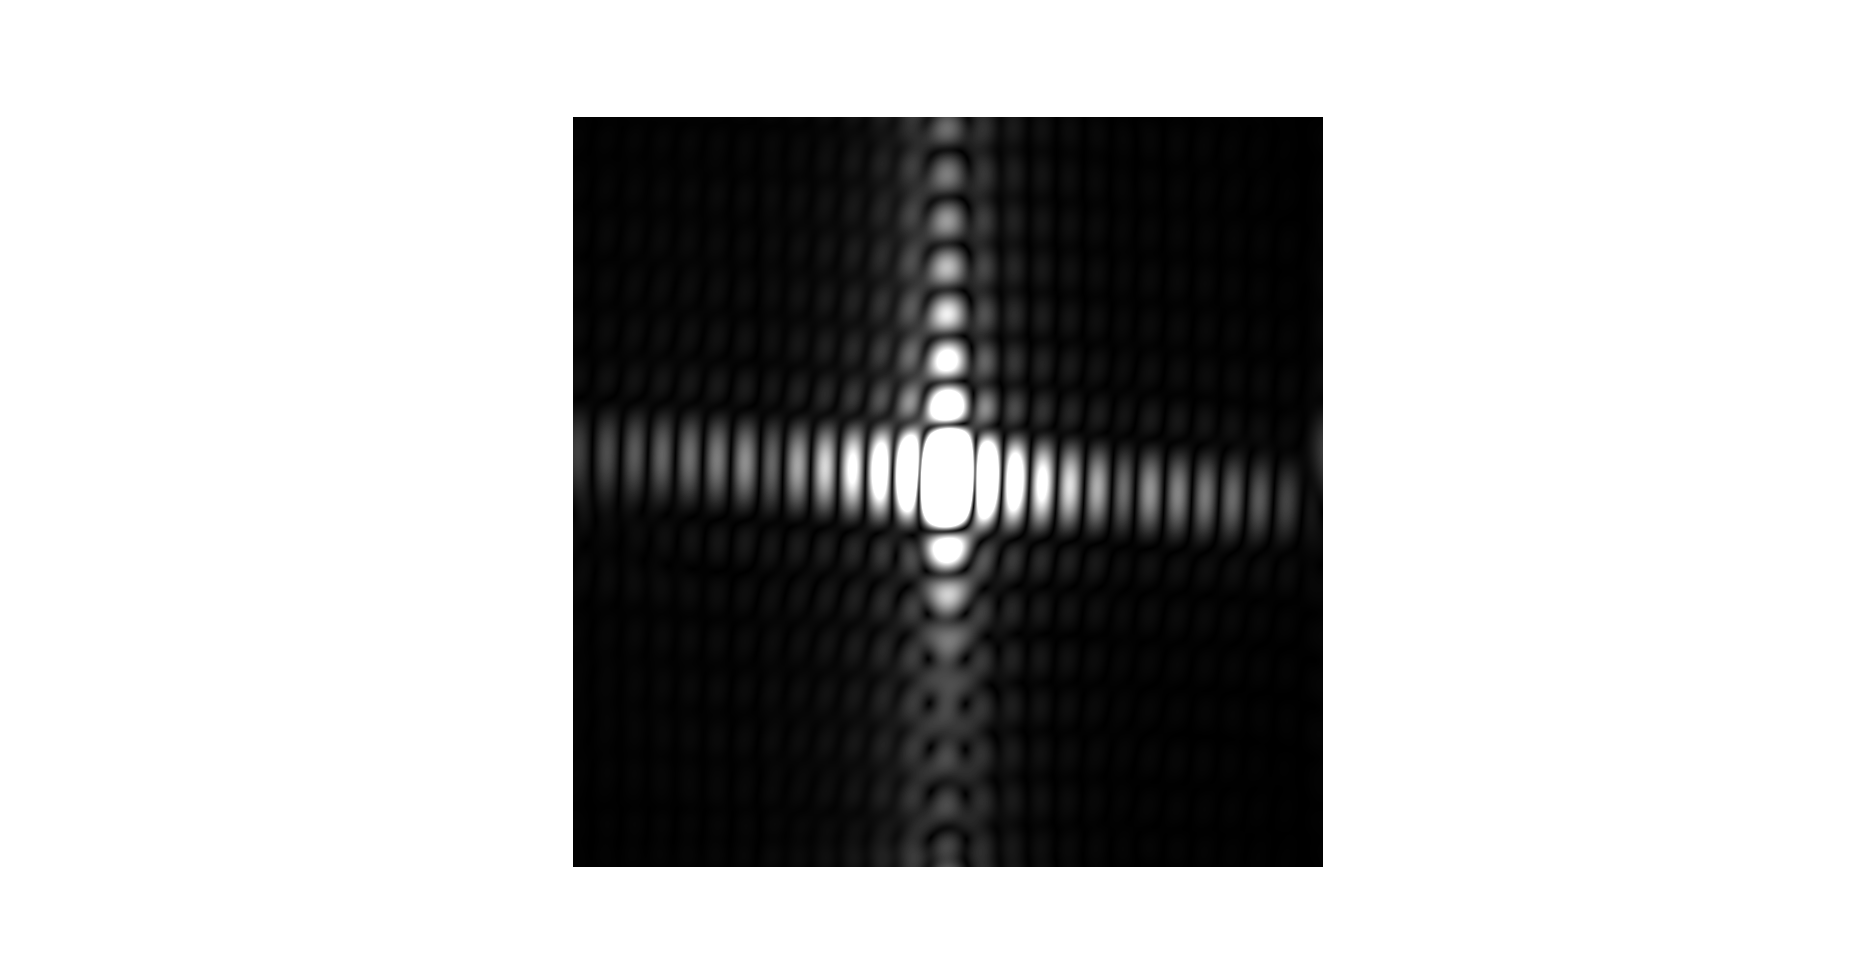
\includegraphics[width=1\textwidth]{point_target.png}
    \caption{Отклик уголкового отражателя}
    \label{fig:point_target}
\end{figure}
	
	Если мы рассчитаем волновой параметр для радиолокатора $ p = \frac{\sqrt{\lambda z}}{b} $, где $ \lambda $ - длина волны, $ z $ - наклонная дальность, $ b $ - линейный размер антенны, то он окажется намного большим 1. Это означает, что мы находимся в области диффрации Фраунгофера. Действительно, если сравнить диффракционную картину Фраунгофера на прямоугольной щели [Сивухин](рисунок \ref{fig:sivukhin}), с изображением отклика от точечной цели (рисунок \ref{fig:point_target}), то можно предположить, что механизм формироания отклика от уголкового отражателя схож с механизмом формировния диффракции, что по сути является проявлением волновой природы света.

\begin{figure}[ht]
    \centering
    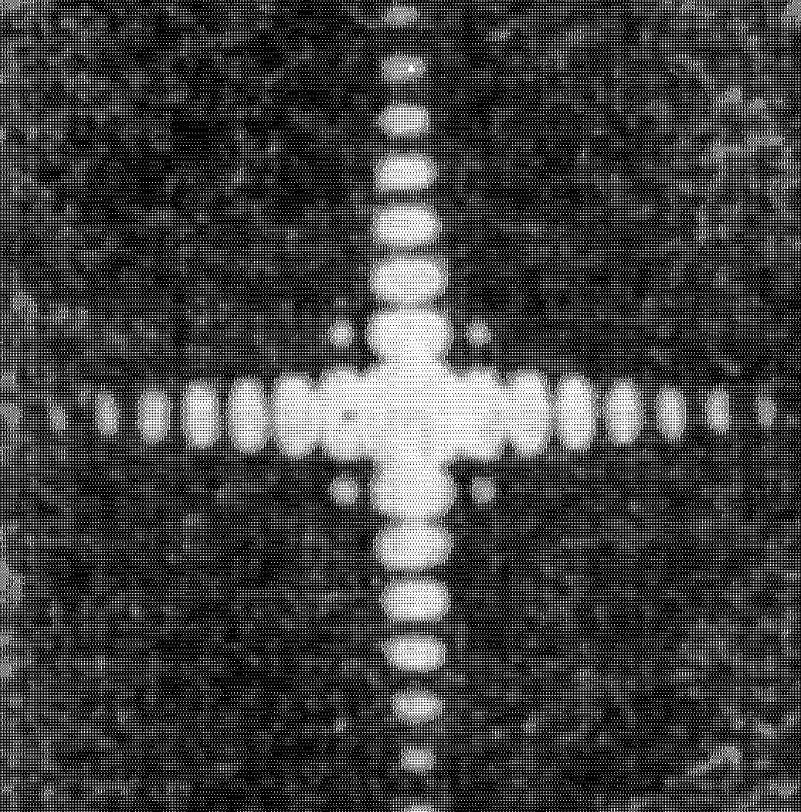
\includegraphics[width=0.4\textwidth]{sivukhin.png}
    \caption{Диффракция Фраунгофера на прямоуголной щели}
    \label{fig:sivukhin}
\end{figure}
	
	Таким образом, можно предположить, что диффракция может происходить не только на уголковых отражателях, но и на других искусственных объектах. Действительно, если взглянуть на РЛИ зданий или кораблей на рисунке \ref{fig:ship_build}, то можно в этом убедиться.
	
\begin{figure}[ht]
    \centering
    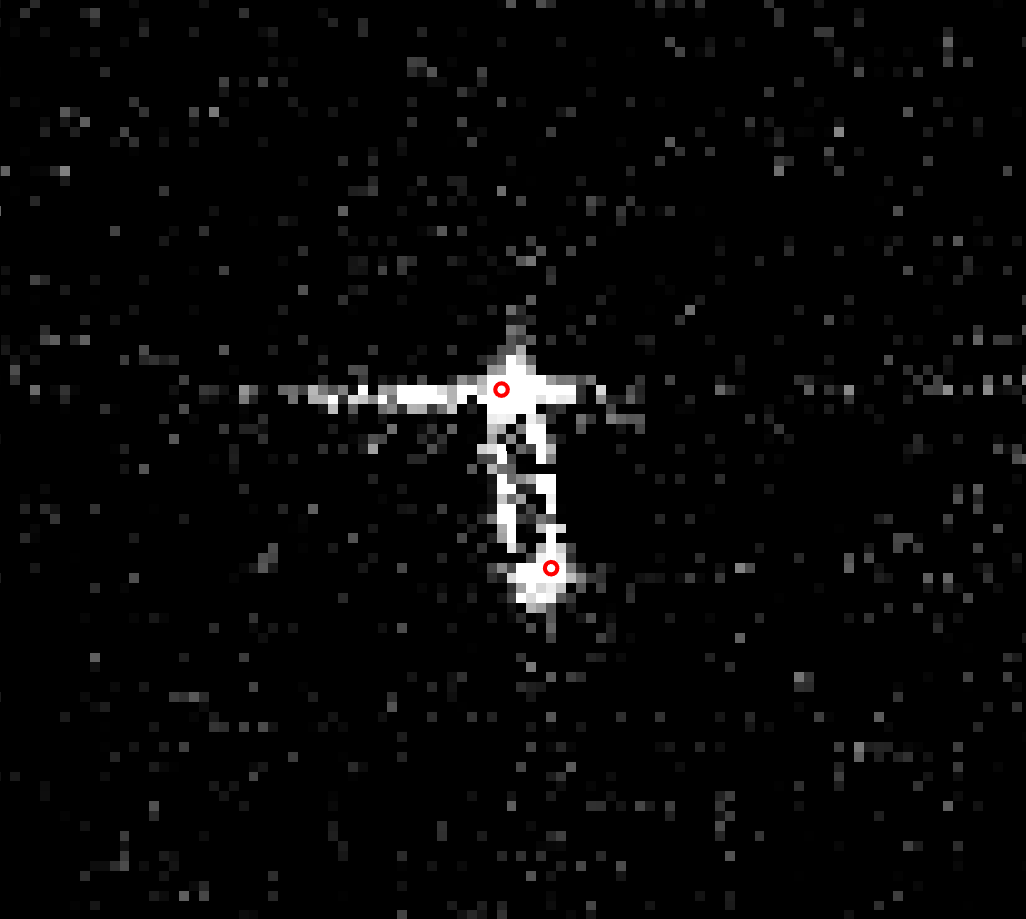
\includegraphics[width=0.4\textwidth]{ship.png}
    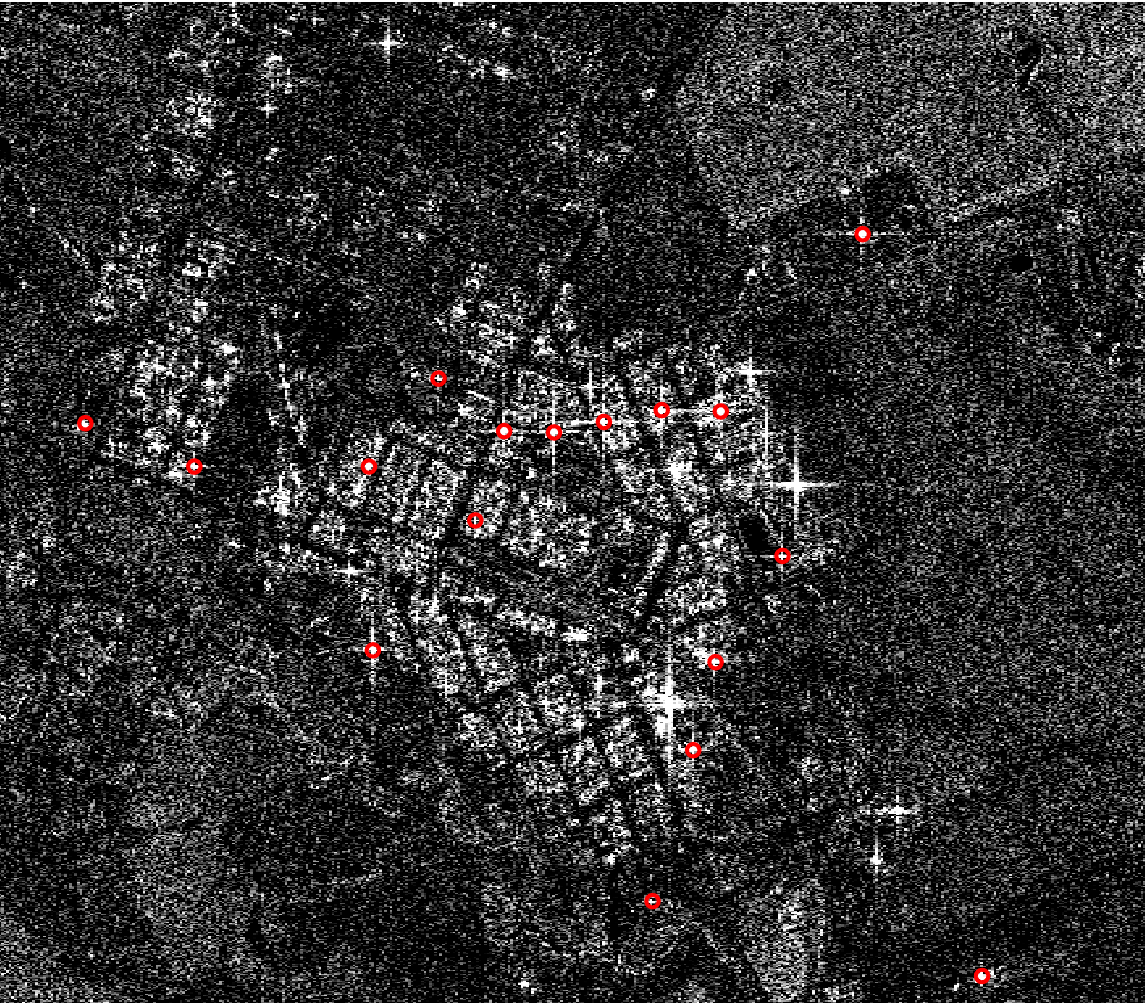
\includegraphics[width=0.4\textwidth]{building.png}
    \caption{РЛИ корабля и зданий}
    \label{fig:ship_build}
\end{figure}
		
	Проблема диффракции на произвольных искусственных объектах заключается в том, что они не являются одиночными, изолированными рассеивателями, то есть не являются точечным целями. По умолчанию отклик от таких объектов будет суммой откликов от точечных целей. И в виду ограниченной разрешающей спсобности радиолокатора они будут сливаться в единую диффракционую картину. Такие объекты, для которых нельзя с полной уверенностью сказать, что они являются одиночными, изолированным рассеивателями, но в тоже время сохраняют диффракционную картину, в данной работе будут называться псевдоточечными целями. 

	Исходя из цели исследования задача данной работы сводится к разработке алгоритма автоматического контроля качества синтеза РЛИ, используя метод анализа отклика от псевдоточечных целей, при отсутствии априорной инфомации о снимаемой сцене. Эффективность разработанного алгоритма будет определятся тем, насколько полученные значения будут отличаться от значений, полученных с помощью точечных целей.

	Таким образом задачи формулируются следующим образом:
	
	1. Разработать алгоритм автоматического поиска псевдоточечных целей на РЛИ
	
	2. Разработать алгоритм анализа отклика от псевдоточечных целей

\newpage
 %% Постановка задачи
    \chapter{Обзор существующих решений}
\label{sec:Chapter2} \index{Chapter2}

Основным критерием поиска подходящего программного обеспечения является его возможность работать с уровнем синтеза  L1, то есть Single Look Complex (SLC). Ниже приведен список приложений для работы с SLC:\\

\section{Открытое программное обеспечения для работы с РЛИ уровня SLC}

1. SNAP - Платформа приложений Sentinel.\\
2. SARscape - это полный набор функций для комплексной обработки всех космических и отдельных авиационных радиолокационных данных.\\
3. GMTSAR - Система обработки InSAR в сочетании с GMT.\\
4. ISCE2 - Научная вычислительная среда InSAR.\\
5. Doris - Делфтское объектно-ориентированное радарно-интерферометрическое программное обеспечение.\\
6. SARPROZ - Инструмент для обработки SAR.\\
7. StaMPS/MTI - Стэнфордский метод для стойких рассеивателей.\\
8. kite - Подвыборка в виде дерева квадрантов, анализ ковариации данных для моделирования смещения поверхности. Удаление точек доступа (эмпирическое и по ДЖЕЙКОБСУ). Загрузка данных из различных центров обработки данных.\\
9. sarpy - Библиотека Python для простой обработки сложных данных SAR с использованием стандарта NGA SIC.\\
10. ROI\_PAC - Sentinel1.\\
11. pygmtsar - Скрипты на Python для обработки GMTSAR.\\
12. Xarray-Sentinel - Серверная часть X-массива для обработки спутниковых данных Copernicus Sentinel-1.\\
13. Sarsen - Алгоритмы и инструменты для геометрической и радиометрической коррекции данных SAR Sentinel-1 с учетом рельефа местности.\\
14. pyroSAR - Фреймворк на Python для крупномасштабной обработки спутниковых данных SAR.\\
15. S1\_NRB - Прототип процессора для радиолокационного устройства с нормализованным обратным рассеянием Sentinel-1.\\
16. ALUs - Различные процессоры, использующие графический процессор, самый быстрый для обеспечения когерентности Sentinel-1 и обратного рассеяния.\\

\subsection{SNAP}
	Главным достоинством SNAP является возможность работы с различными пакетами данных с разных спутников. Также присутствуют инструменты для работы с шумами, геопривязкой, поляризационными изображениями. Есть все функции для постобработки изображений.\\
	
	
\begin{figure}[ht]
    \centering
    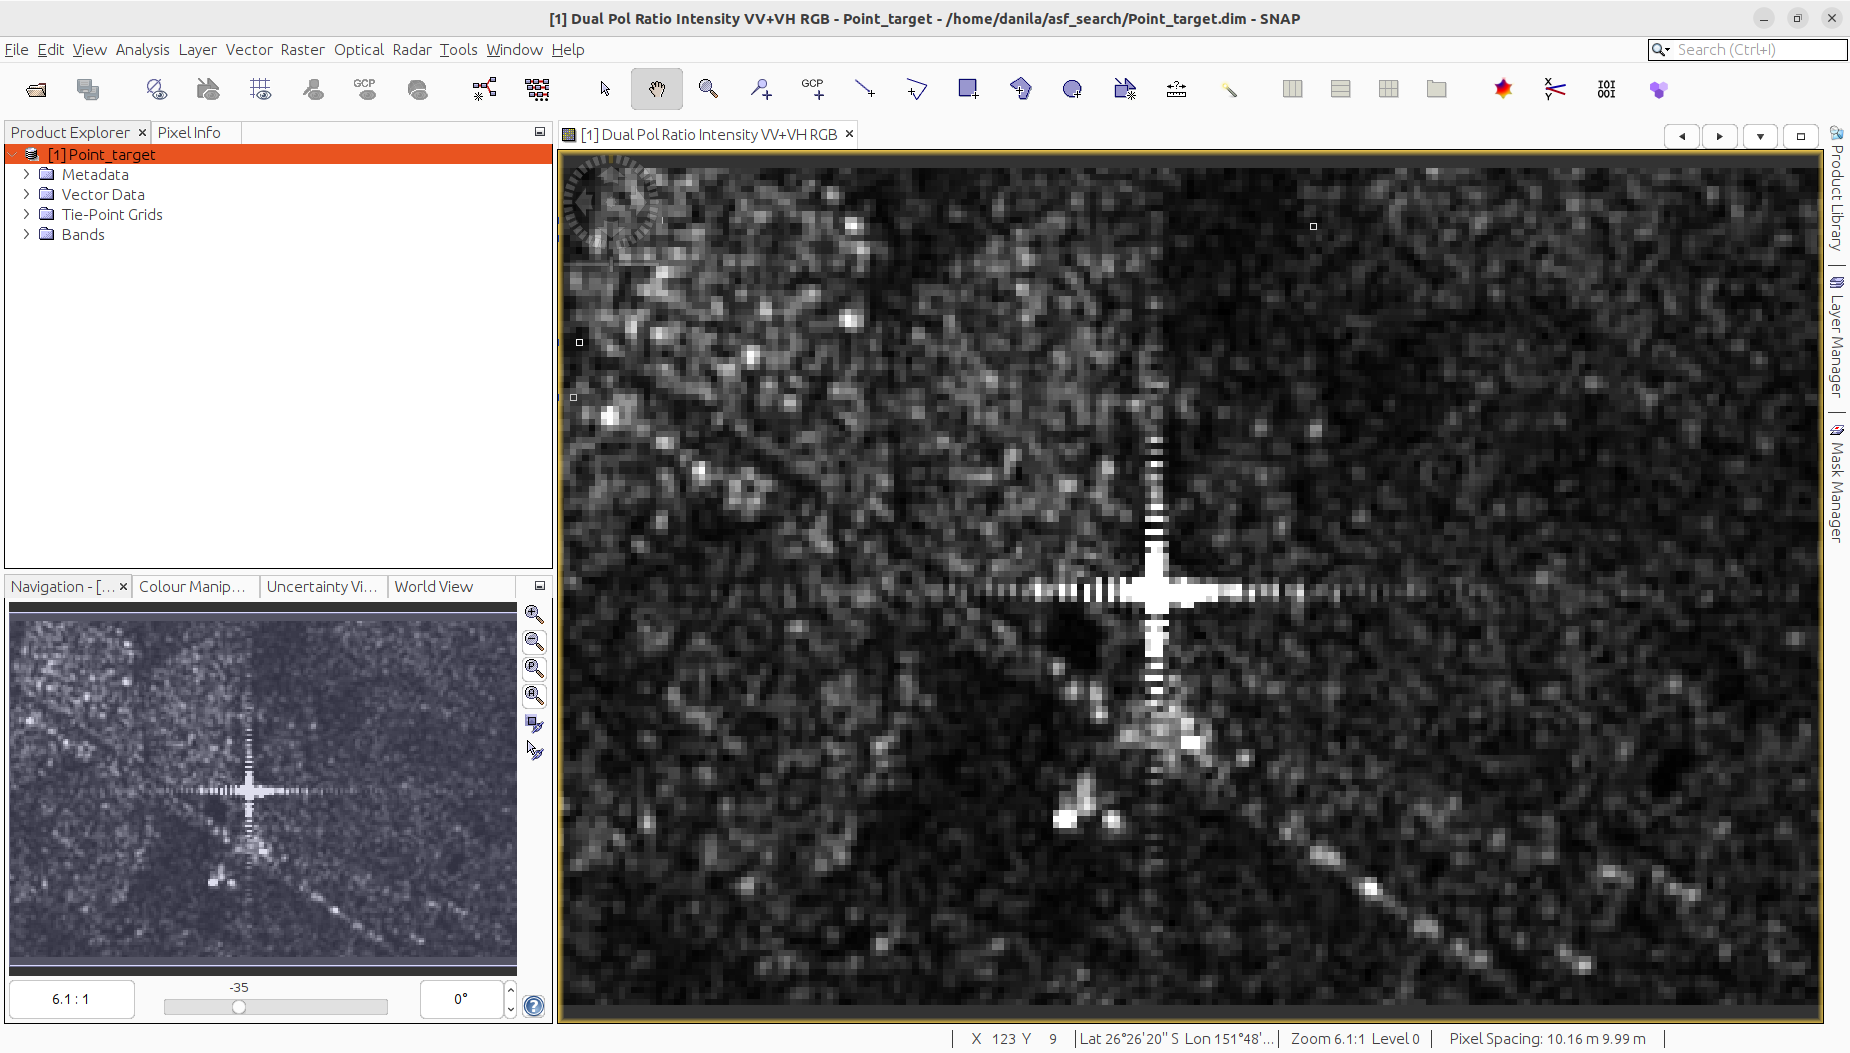
\includegraphics[width=0.8\textwidth]{snap.png}
    \caption{SNAP}
    \label{fig:snap}
\end{figure}

	
\subsection{SARscape}
	В данный момент приложение SARscape не доступно в России. Поэтому анализ невозможен.\\
	
\subsection{GMTSAR}		
	Данное программное обеспечение предоставляет возможности синтеза и постобработки изображений без графического интерфейса. Также присутсвуют функции для интерферометрической обработки.\\
	
\subsection{SARPROZ}
	Богатый функционал для работы с РЛИ уровня SLC.\\	

\begin{figure}[ht]
    \centering
    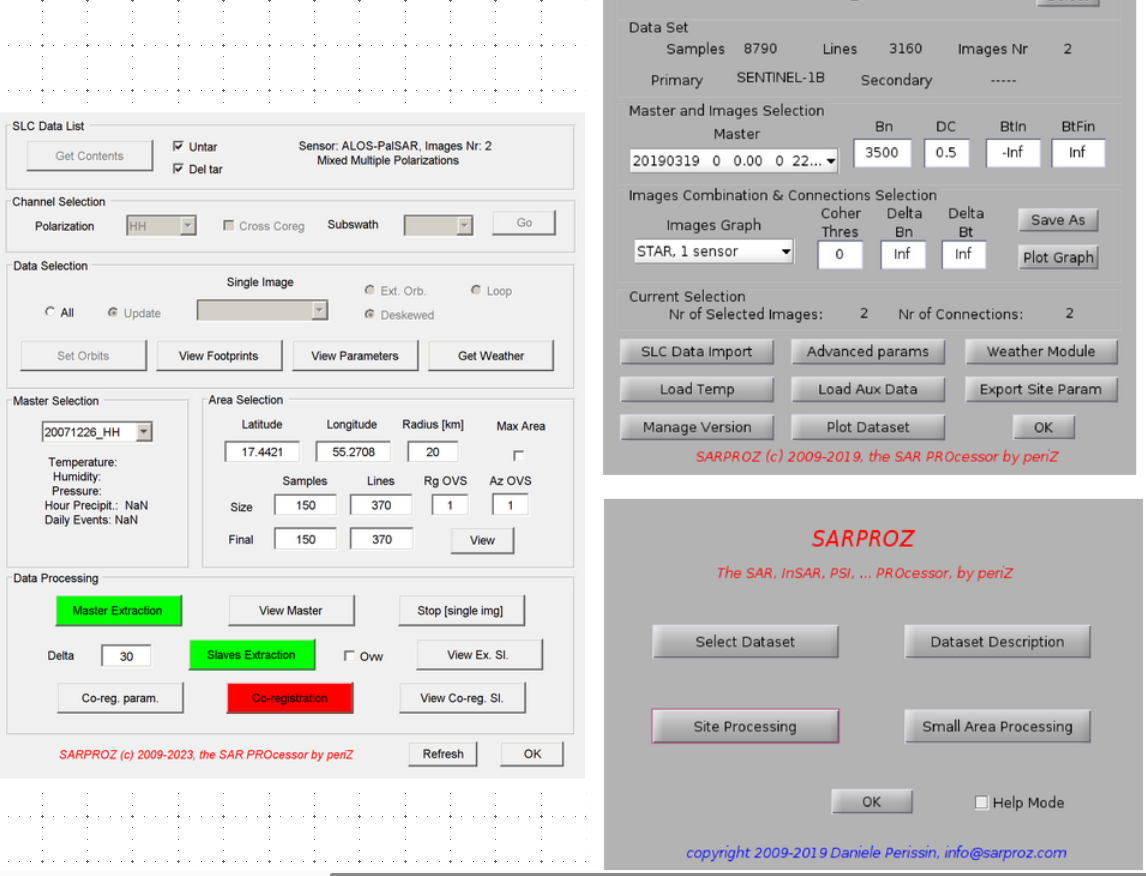
\includegraphics[width=0.8\textwidth]{sarproz.png}
    \caption{SARPROZ}
    \label{fig:sarproz}
\end{figure}
	
\subsection{StaMPS/MTI}

\section{Выводы}

	Все представленные выше программные комплексы не имеют возможности оценки разрешения РЛИ по точечным целям. Исключение составляет Radar Tools (RAT), но данное приложение написано на языке Interactive Data Language (IDL), лецензию на который невозможно получить из России. Также существует платформа SARvis, упомянутое в статье [], в котором также присутсвуют инструменты для определния разрешений РЛИ. Но найти данное приложение в открытом доступе не удалось
	
\newpage
 %% Обзор существующих решений
    \chapter{Исследование и построение решения задачи}
\label{sec:Chapter3} \index{Chapter3}


\section{Показатели качества РЛИ}

	Важным показателем качества синтеза РЛИ является пространственное разрешение, которое характеризует наименьшее расстояние для раздельного воспроизведения изображения двух точечных объектов. При разнесении точек в пространстве посередине между ними в изображении возникает локальный минимум интенсивности (провал). Разрешение определяется величиной наименьшего расстояния, на котором достоверно обнаруживается этот провал [Занин]:
	
\begin{equation}
    \Delta y = k_p*R_g,
\end{equation}

где $ \Delta y $ - расстояние между точечными объектами (линейное разрешение), $ k_p $ - коэффициент ухудшения разрешения относительно идеального, $ R_g $ - предельная разрешающая способность РСА. 
	Данное расстояние зависит от контраста наблюдаемого объекта, отношения сигнал-шум и ошибок информационного тракта. Целью синтеза РЛИ является сделать пространственное разрешение равным предельной разрешающей способности РСА.
	
	Общепринятым подходом для оценки разрешения РЛИ является измерение ширины профиля квадрата функции рассеяния точки (ФРТ) по уровню -3 дБ в направлениях азимута и дальности. Также существуют и другие методы, такие как измерение пространственного разрешения по автокорреляционной функции  изображения [2], оценка разрешения по протяженным линейным объектам [2], использование элементов алгоритма PGA [2]. Также в [] предложено измерять разрешение по формуле:
	
\begin{equation}
    \Delta y = k_p*R_g,
\end{equation}
	
	Помимо этого в [] предложено измерять разрешение по периодическим структурам.	
	
	Преимуществом анализа ФРТ является то, что помимо разрешения, с помощью него можно вычислить и другие параметры РЛИ, такие как контраст, отношение сигнал/шум и др. Так как радиолокационые системы (РЛС) являются линейными [1 с.59 Wong], то есть вид их передаточных функций не зависит от величины входного воздействия, то естественно исследовать ФРТ как отклик от единичного импульса, который формируется тест объектом. В РСА таким тест объектом является одиночный, изолированный рассеиватель, такой как уголковый отражатель. Особенность его заключается в том, что падающий на него зондирующий импульс отражается точно в противоположном направлении. Такой малый, дискретный рассеиватель ещё называют точечной целью. Большинство параметров РЛС измеряются по отклику от такой цели. Откликом точечной цели является sinc-like функция [1].

	Идея данной работы заключается в использовании в качестве тест объектов псевдоточечные цели, то есть цели, для которых заведомо неизвестно, являются ли они одиночными, изолированными, то есть точечными. При большой выборке данных целей (100 - 1000 штук), в ней могут оказаться как точечные, так и неточечные. Соответсвенно профиль функции рассеяния псевдоточечной цели будет шире чем профиль ФРТ, так как функция рассеяния псевдоточечной цели будет суммой ФРТ, сдвинутых друг относительно друга на $ {\delta x < \Delta y} $. 

	Далее рассмотрим механизм формирования отклика от псевдоточечной цели. Логично, предположить, что данный отклик будет суммой откликов от точечных целей, раз мы считаем точечную цель неделимой, единичной структурой.
	
\section{Модель формирования псевдоточечных целей}

	Точечные цели образуют псевдоточечные цели, если они расположены на расстоянии меньше разрешающей способности радиолокатора. Возьмём точечные цели с разрешением 0.8838 м и расположим случайным образом на фиксированной сцене. Геометрия получившейся модели показана на рисунке \ref{fig:pseudo_targets}.
	
	
\begin{figure}[ht]
    \centering
    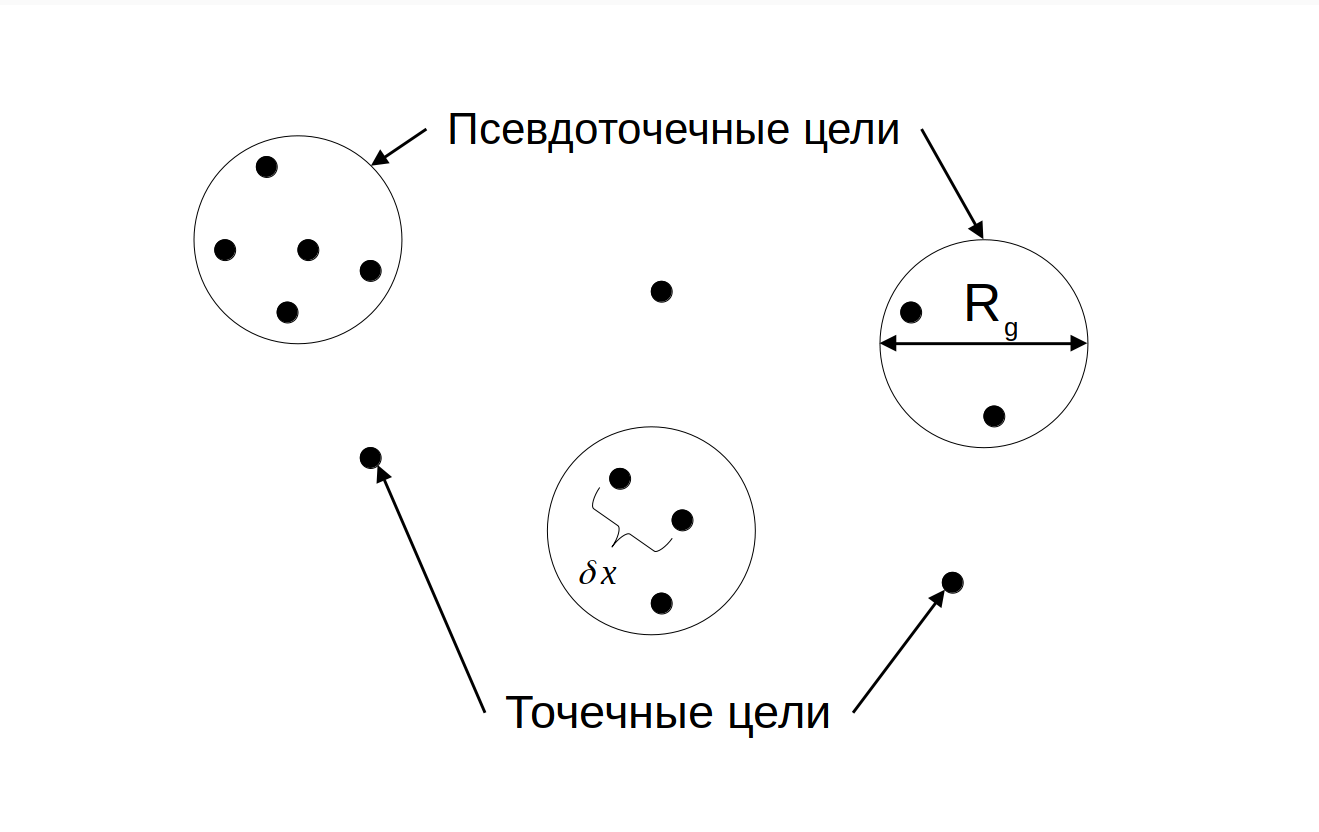
\includegraphics[width=0.8\textwidth]{pseudo_targets.png}
    \caption{Модель формировния псевдоточечных целей}
    \label{fig:pseudo_targets}
\end{figure}


	Те точечные цели, что попали в круг радиуса  $R_g$  (разрешающей способности радиолокатора) , образует единый отклик псевдоточечной цели. Сгенерируем случайным образом отклонения $ \delta x $ и количество попавших в круг целей и рассчитаем разрешения получившихся псевдоточечных целей. После этого найдем максимум распределения. Код модели, реализованный на языке Python 3 представлен ниже.
	
\begin{verbatim}
	import matplotlib.pyplot as plt
	import numpy as np
	from scipy.signal import find_peaks
	from scipy.signal import peak_widths

	def point_target(x, a):
	    """
	    Вычисляет квадрат отклика точеченой цели
	    :param x: массив действительных чисел, числовая ось
	    :param a: параметр, отвечающий за разрешение
	    :return: массив отклика точечной цели
	    """
	    arg = np.pi*x/a
	    return pow(np.sin(arg)/arg, 2)

	def irw(signal):
	    """
	    Вычисляет IRW (impulse response width) входного сигнала
	    :param signal: массив действительных чисел, функция вида sin(x)/x
	    :return: значение IRW сигнала
	    """
	    # Находим локальные максимумы
	    peaks = find_peaks(signal)[0]
	    # Мерим их ширину на высоте 1/sqrt(2)
	    width = peak_widths(signal, peaks, rel_height=1 - pow(10, -0.3))[0]
	    # Отбираем максимальную ширину - ширину главного лепестка
	    irw = np.max(width)
	    return irw

	def max_distr(arr):
	    """
	    Вычисляет максимум распределения массива arr
	    :param arr: массив действительных чисел
	    :return: максимум распределения
	    """
	    arr.sort()    
	    while len(arr) > 1:    
		border = (arr[0] + arr[-1])/2       
		if all([x == border for x in arr]):
		    break            
		left = []
		right = []        
		for item in arr:
		    if item < border:
		        left.append(item)
		    else:
		        right.append(item)            
		if len(right) > len(left):
		    arr = right
		else:
		    arr = left		    
	    return arr[0]
		
	a = 1 
	start = -10
	stop = 10
	count = 1000
	scale = (stop - start)/count

	t = np.linspace(start, stop, count)

	dx = np.random.rand(1000)
	dx = (2*dx - 1)*a
	res = []

	for n in np.random.randint(1, 10, 1000):
	    s = [0]*len(t)
	    for delta in np.random.choice(dx, n):
		s += point_target(t + delta, a)        
	    res.append(scale*irw(s))

	print("Разрешение точечной цели:",  round(scale*irw(point_target(t, a)), 4))
	print("Максимум распределения разрешений псевдоточечных целей", round(max_distr(res), 4))
\end{verbatim}

	График получившегося распределния представлен нна рисунке \ref{fig:pseudo_distr}.

\begin{figure}[ht]
    \centering
    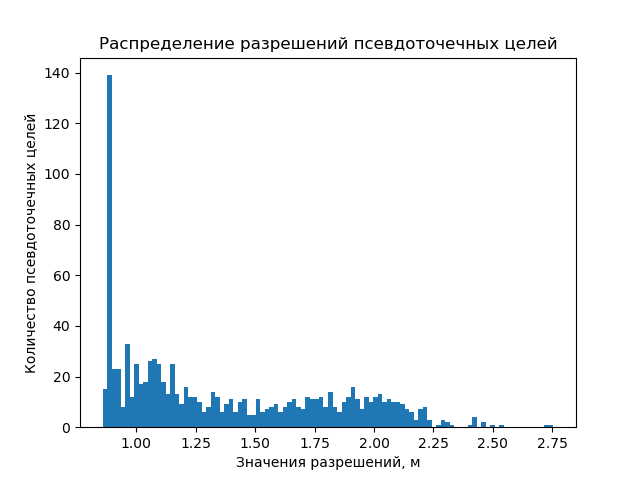
\includegraphics[width=0.8\textwidth]{pseudo_distr.png}
    \caption{Гистограмма распределния разрешений псевдоточечных целей}
    \label{fig:pseudo_distr}
\end{figure}

	Таким образом, максимум распределения разрешений псевдоточечных целей оказалось равно 0.8836, что отличается от эталонного не более чем на 0.03\%. Исходя из этого можно сделать вывод, что статистический анализ псевдоточечных целей даёт результаты очень близкие к реальным.

\section{Алгоритм поиска псевдоточечных целей на РЛИ}

	Алгоритм автоматического поиска псевдоточечных целей заключается в нахождении центров их откликов. В [Automatic point...] предложен алгоритм поиска, который заключается в вычислении свертки областей РЛИ с заранее сгенерированными квадратными матрицами, которые задают направления "лучей" отклика. У него есть ряд недостатков:
	
	1. Свертка применяется ко всем областям РЛИ
	
	2. Заранее сгенерированные матрицы имеют ограниченное количество направлений
	
	Данные проблемы решаются с помощью выделения наиболее информативных областей и использовании в качестве свёрточных матриц автокорреляционную функцию изображения.

\subsection{Выделение информативных участков изображения}

	Вычисление свёртки - ресурсозатратная операция для компьютера. Нецелесообразно производить вычисления на областях с высоким уровнем шума или на слабоотражающих участках, так как результат свёртки будет неопределен. Для первичной фильтрации входного изображения используются гистограммные признаки [prett]. В начале входное изображение разбивается на равные участки путем создания двумерной сетки. Далее для каждого участка вычисляется гистограммный признак и на основании его значения делается вывод. Всего было протестировано 6 признаков: среднее, дисперсия, коэффициент асимметрии, кожффициент эксцесса, энергия, энтропия. Однако наибольшей информативностью обладает коэффициент эксцесса. Данный вывод был сделан на основе решения задачи бинарной классификация, где правилом классификации выступало отклонение разрешения псевдоточечной цели от истинной. Таким образом, удалось выяснить, что на участках изображения со значением коэффициента эксцеса больше 10 имеют с большей вероятностью могут находится псевдоточечные цели с разрешением, близким к истинному. Результат бинарной классификации представлен на рисунке \ref{fig:binary_classification}, где зелеными звездочками помечены те учатки изображения, на которых имеются уголковые отражатели. 
	
\begin{figure}[ht]
    \centering
    
\includegraphics[width=0.8\textwidth]{binary_classification.png}
    \caption{Бинарная классификация}
    \label{fig:binary_classification}
\end{figure}

\subsection{Свёрточная матрица на основе автокорреляционной функции изображения}

	Вычисление автокорреляционной функции (АКФ) является ключевым элементом в обработке РЛИ: она используется для оценки разрешающей способности РСА, в методе автофокусировки, в оценке когерентности и шумов. По определению автокорреляционная функция комплексного изображения задается формулой:
	
\begin{equation}
    R_{II}(\Delta x, \Delta y) = \iint_{-\infty}^{\infty} I(x, y) \cdot I^*(x - \Delta x, y - \Delta y) \, dx \, dy
\end{equation}

где:
\begin{itemize}
	\item $I(x, y)$ - комплексное изображение,
	\item $I^*(x - \Delta x, y - \Delta y)$ - комплексно сопряженное изображение, сдвинутое на $(\Delta x, \Delta y)$,
	\item $\Delta x, \Delta y$ - пространственные сдвиги по осям $x$ и $y$ соответственно.
\end{itemize}

	На практике АКФ часто вычисляется через быстрое преобразование Фурье (БПФ) для ускорения расчётов:

	1. Вычисляется Фурье-образ изображения \(\mathcal{F}\{I\}\).
	2. Находится спектр мощности: \(S = |\mathcal{F}\{I\}|^2\).
	3. Обратное Фурье0преобразование от \(S\) даёт АКФ
	
	Или же сокращенно:
	
\begin{equation}
    \text{АКФ} = \mathrm{IFFT}(|\mathrm{FFT}(I)|^2)
\end{equation}	

	В радиолокации существует глубокая аналогия между АКФ и ФРТ. Обе функции описывают пространственное распределение энергии волнового фронта после взаимодействия с системой.
	
	ФРТ описывается функцией sinc:
	
\begin{equation}
    I(\theta) \sim \text{sinc}^2\left(\frac{\pi L \sin\theta}{\lambda}\right)
\end{equation}

	АКФ линейно-частотно модулированного (ЛЧМ) сигнала с полосой B:
	
\begin{equation}
    R{\tau} \sim \text{sinc}(\pi B \tau)
\end{equation}

	Пространственное разрешение обратно пропорциональна шиирине главного лепестка АКФ, что верно и для ФРТ. Таким образом, корреляция между ФРТ и АКФ будет иметь значение близкое к 1. Поэтому целесообразно использовать АКФ как свёрточную матрицу для нахождения псевдоточечных целей. Примеры АКФ и ФРТ предствалены на рисунках \ref{fig:acf} и ...:
	

\begin{figure}[ht]
    \centering
    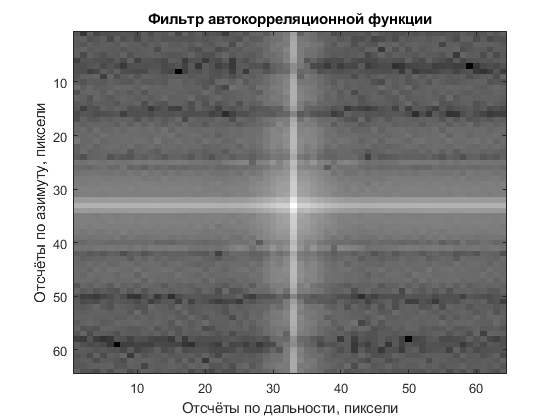
\includegraphics[width=0.8\textwidth]{acf.png}
    \caption{Автокорреляционная функция}
    \label{fig:acf}
\end{figure}


	При повороте точечной цели на некоторый угол, её АКФ также поворачивается, что позволяет учесть всевозможные напрвления "лучей". 	

\subsection{Алгоритм поиска псевдоточечных целей}

	На рисунке \ref{fig:alg_search_targets} представлена блок-схема алгоритма поиска псевдоточечных целей:

\begin{figure}[ht]
    \centering
    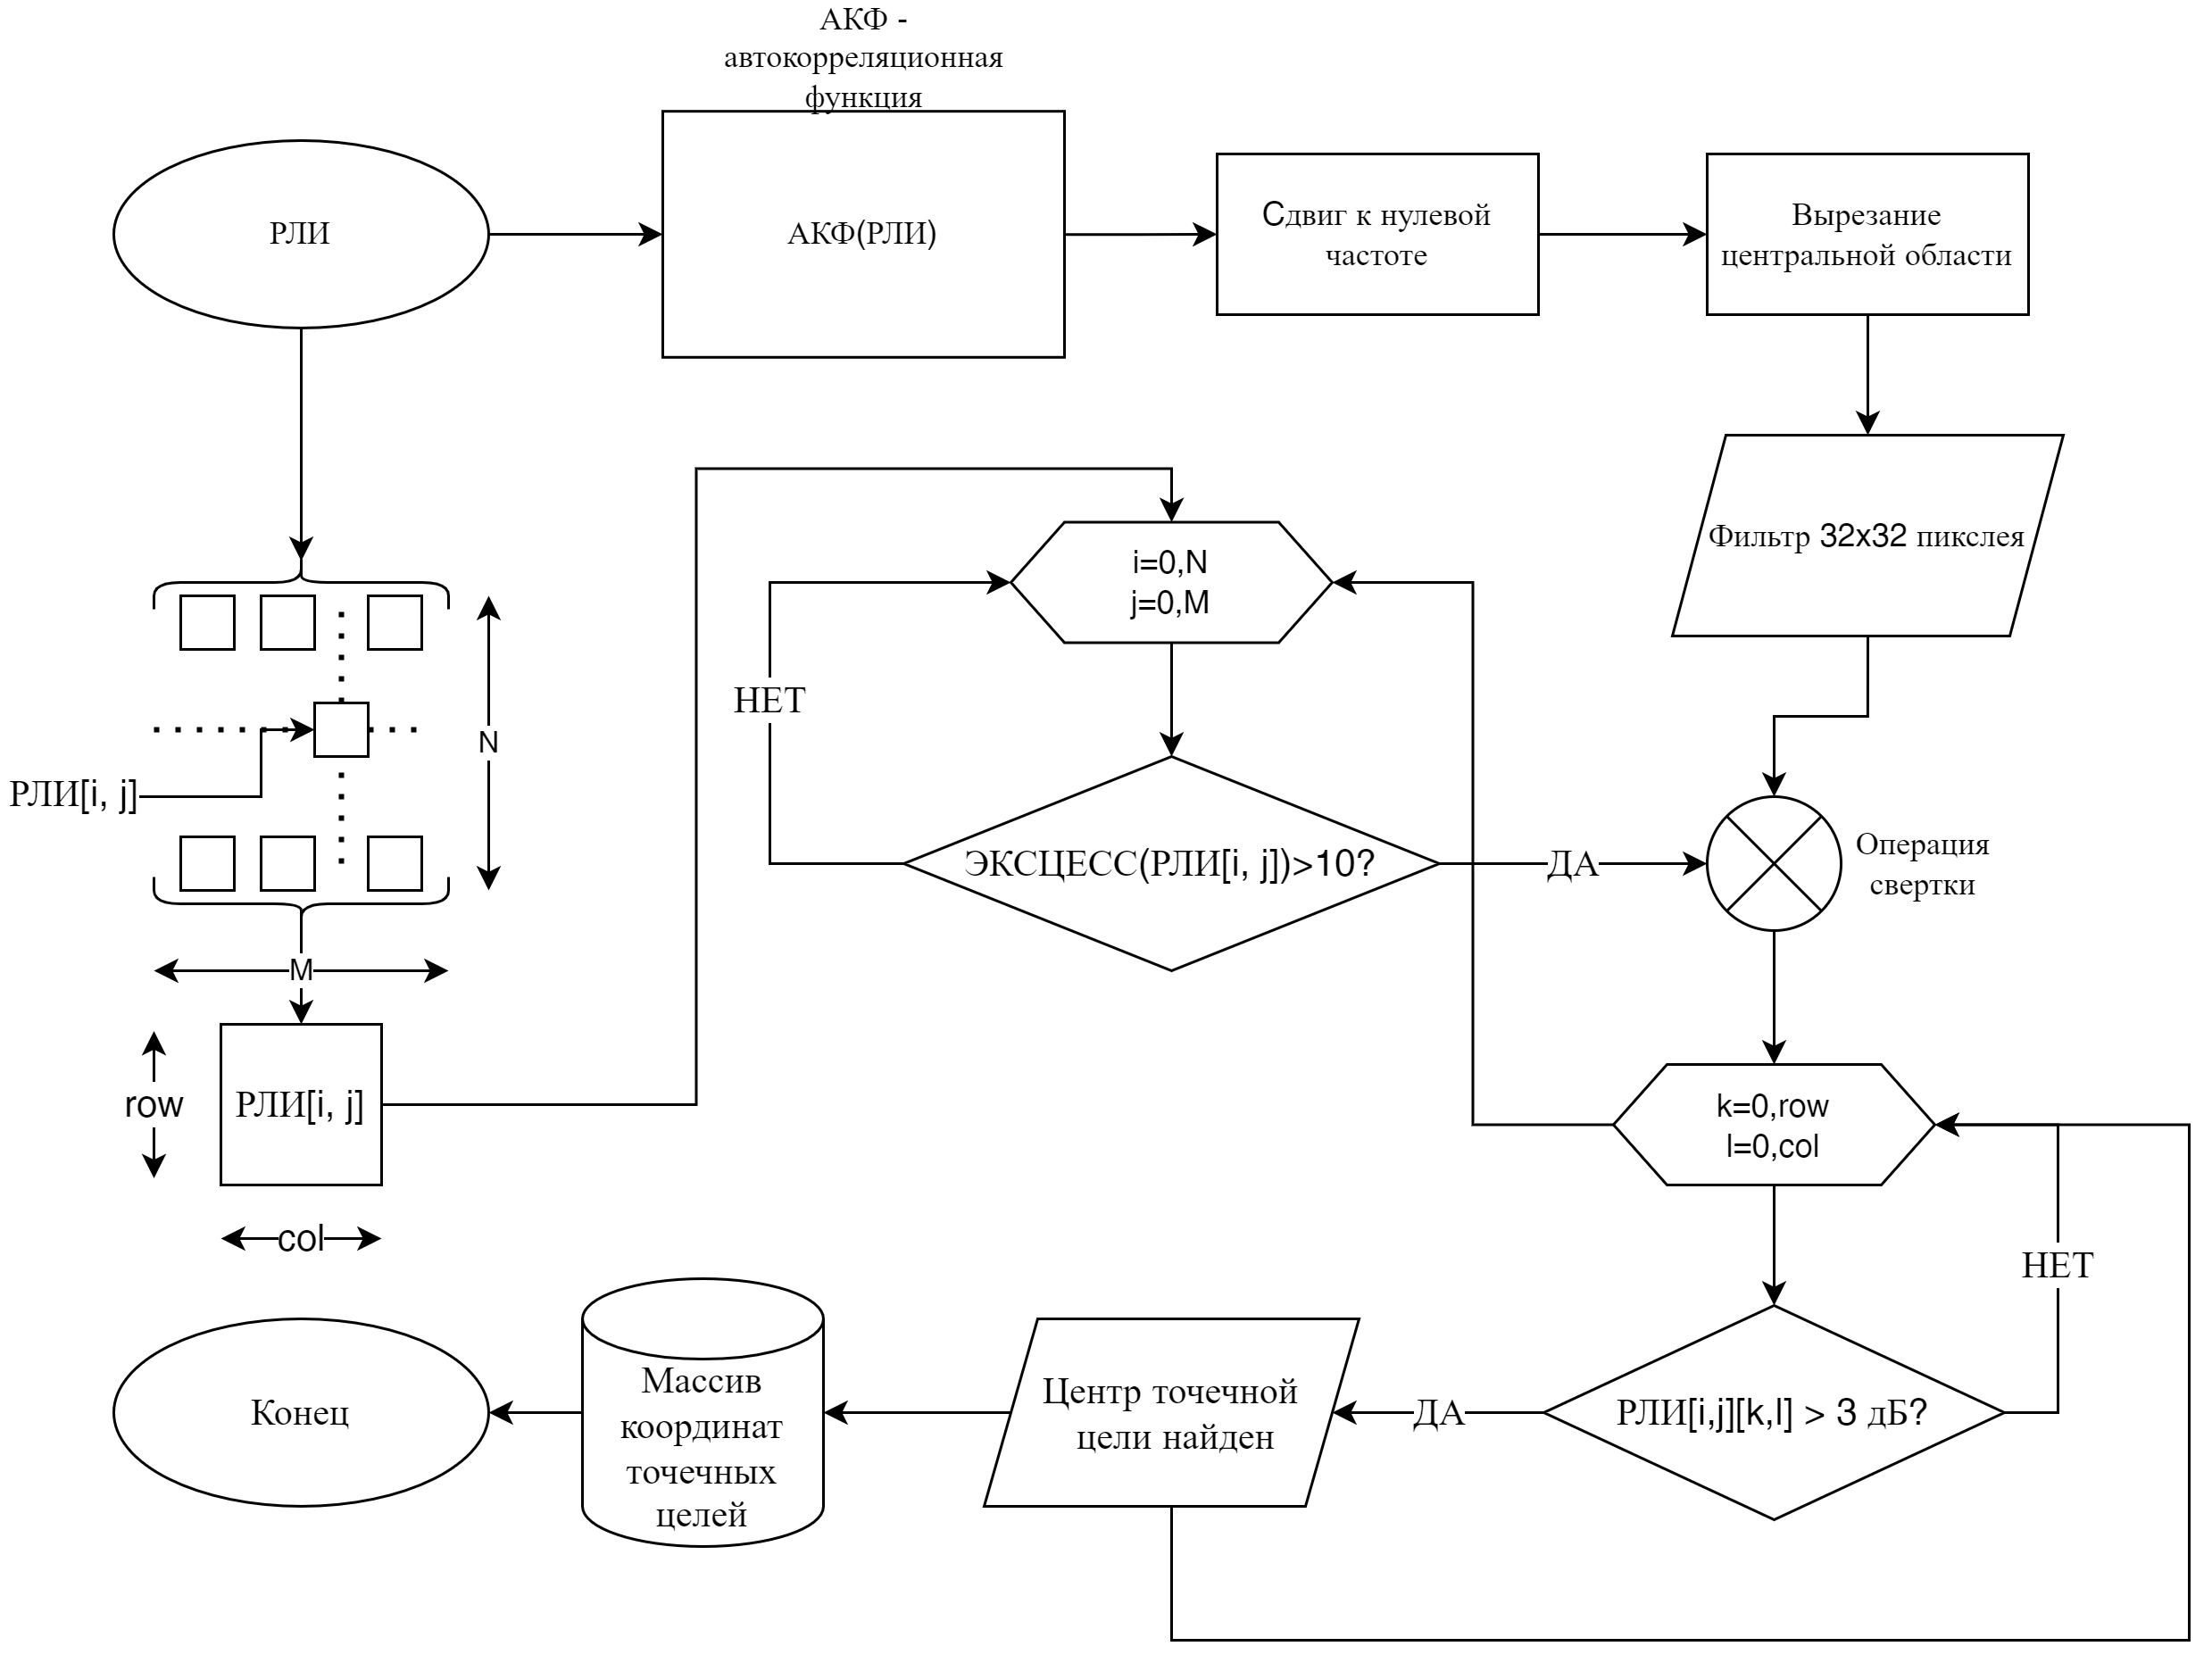
\includegraphics[width=1\textwidth]{alg_search_targets.png}
    \caption{Алгоритм поиска псевдоточечных целей}
    \label{fig:alg_search_targets}
\end{figure}

Она состоит из следующих шагов:

	1) Создание фильтра на основе автокорелляционной функции изображения
	
	2) Создание сетки на изображении с адаптивным шагом
	
	3) Вычисление статистического коэффициента ЭКСЦЕСС
	
	4) Отбор нужных клеток сетки по критерию ЭСЦЕСС > 10
	
	5) Вычисление свертки фильтра, полученного на 1 шаге, и отобранных областей
	
	6) Отбор значений пикселей по пороговому значению (данные пиксели являются центром точечных отражателей)

	Новизна представленного алгоритма заключается в использовании в качестве фильтра центр автокорреляционной функции изображения. Далее выполняется свёртка этого фильтра с наиболее информативными участками изображения. Это означает, что зашумленные или слабоотражающие участки нас не интересует, так как свертка с ними даст неопределенный результат. Поэтому для выделения наиболее информативных участков изображения используется статистический коэффициент ЭКСЦЕСС. Его особенность заключается в том, что он стремится к нулю при гауссовом распределении. Также была решена задача бинарной классификации, которая показала, что участки изображения с точечными целями c хорошим отношением сишнал/шум имеют значения ЭКСЦЕССА > 10. Далее после выполнения операции свертки пиксели отбираются по пороговому значению, это и будут центры точечных отражателей.		

\section{Алгоритм анализа отклика от псевдоточечных целей}

	Алгоритм анализа отклика от псевдоточечных целей ничем не отличается от анализа отклика от точечных целей. Согласно [Wong] наиболее важными характеристиками являются IRW (ширина главного лепестка по уровню -3дБ), PSLR (пиковый уровень боковых лепестков) и ISLR (интегральный уровень боковых лепестков). IRW явлется пространственным разрешением, а ISLR и PSLR отвечают за контраст.  
	

\begin{figure}[ht]
    \centering
    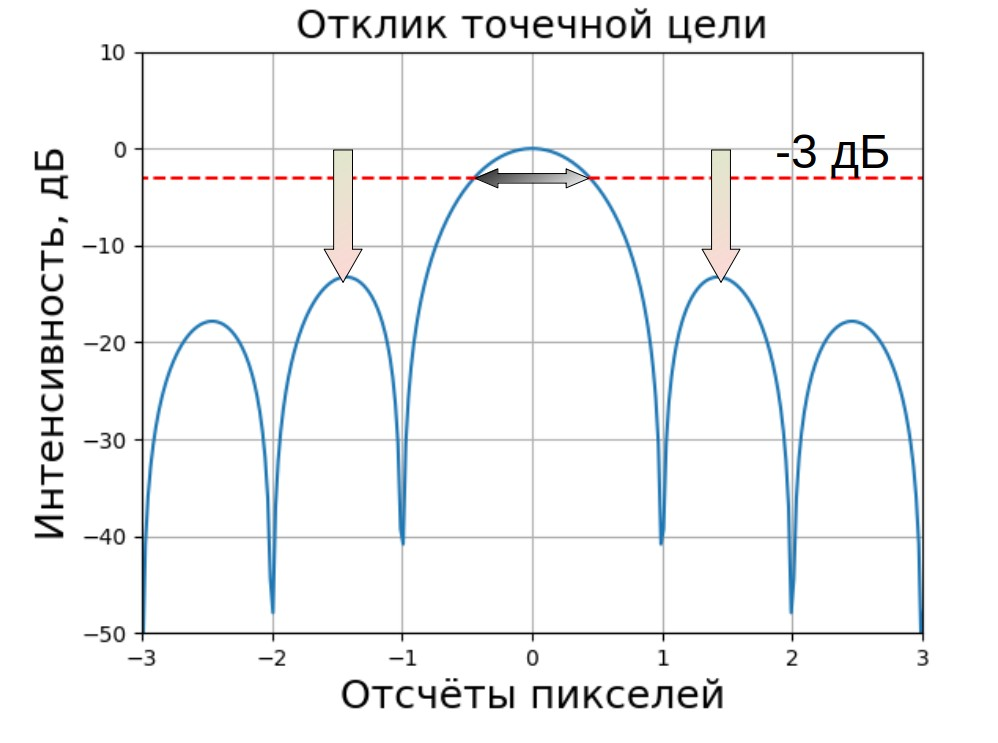
\includegraphics[width=0.8\textwidth]{metrics.png}
    \caption{Измерение характеристик по функции отклика}
    \label{fig:metrics}
\end{figure}
	
	На рисунке \ref{fig:alg_analys_targets} представлена блок-схема алгоритма анализа псевдоточечных целей. Она состоит из следующих шагов:
	
	1. Интерполяция исходного отклика методом добавления нулей в конец спектра.
	
	2. Определение направляющих осей по азимуту и по дальности.
	
	3. Вычисление проекции отклика на данные оси
	
	4. Расчёт требуемых характеристик по даннным проекциям
	
\begin{figure}[ht]
    \centering
    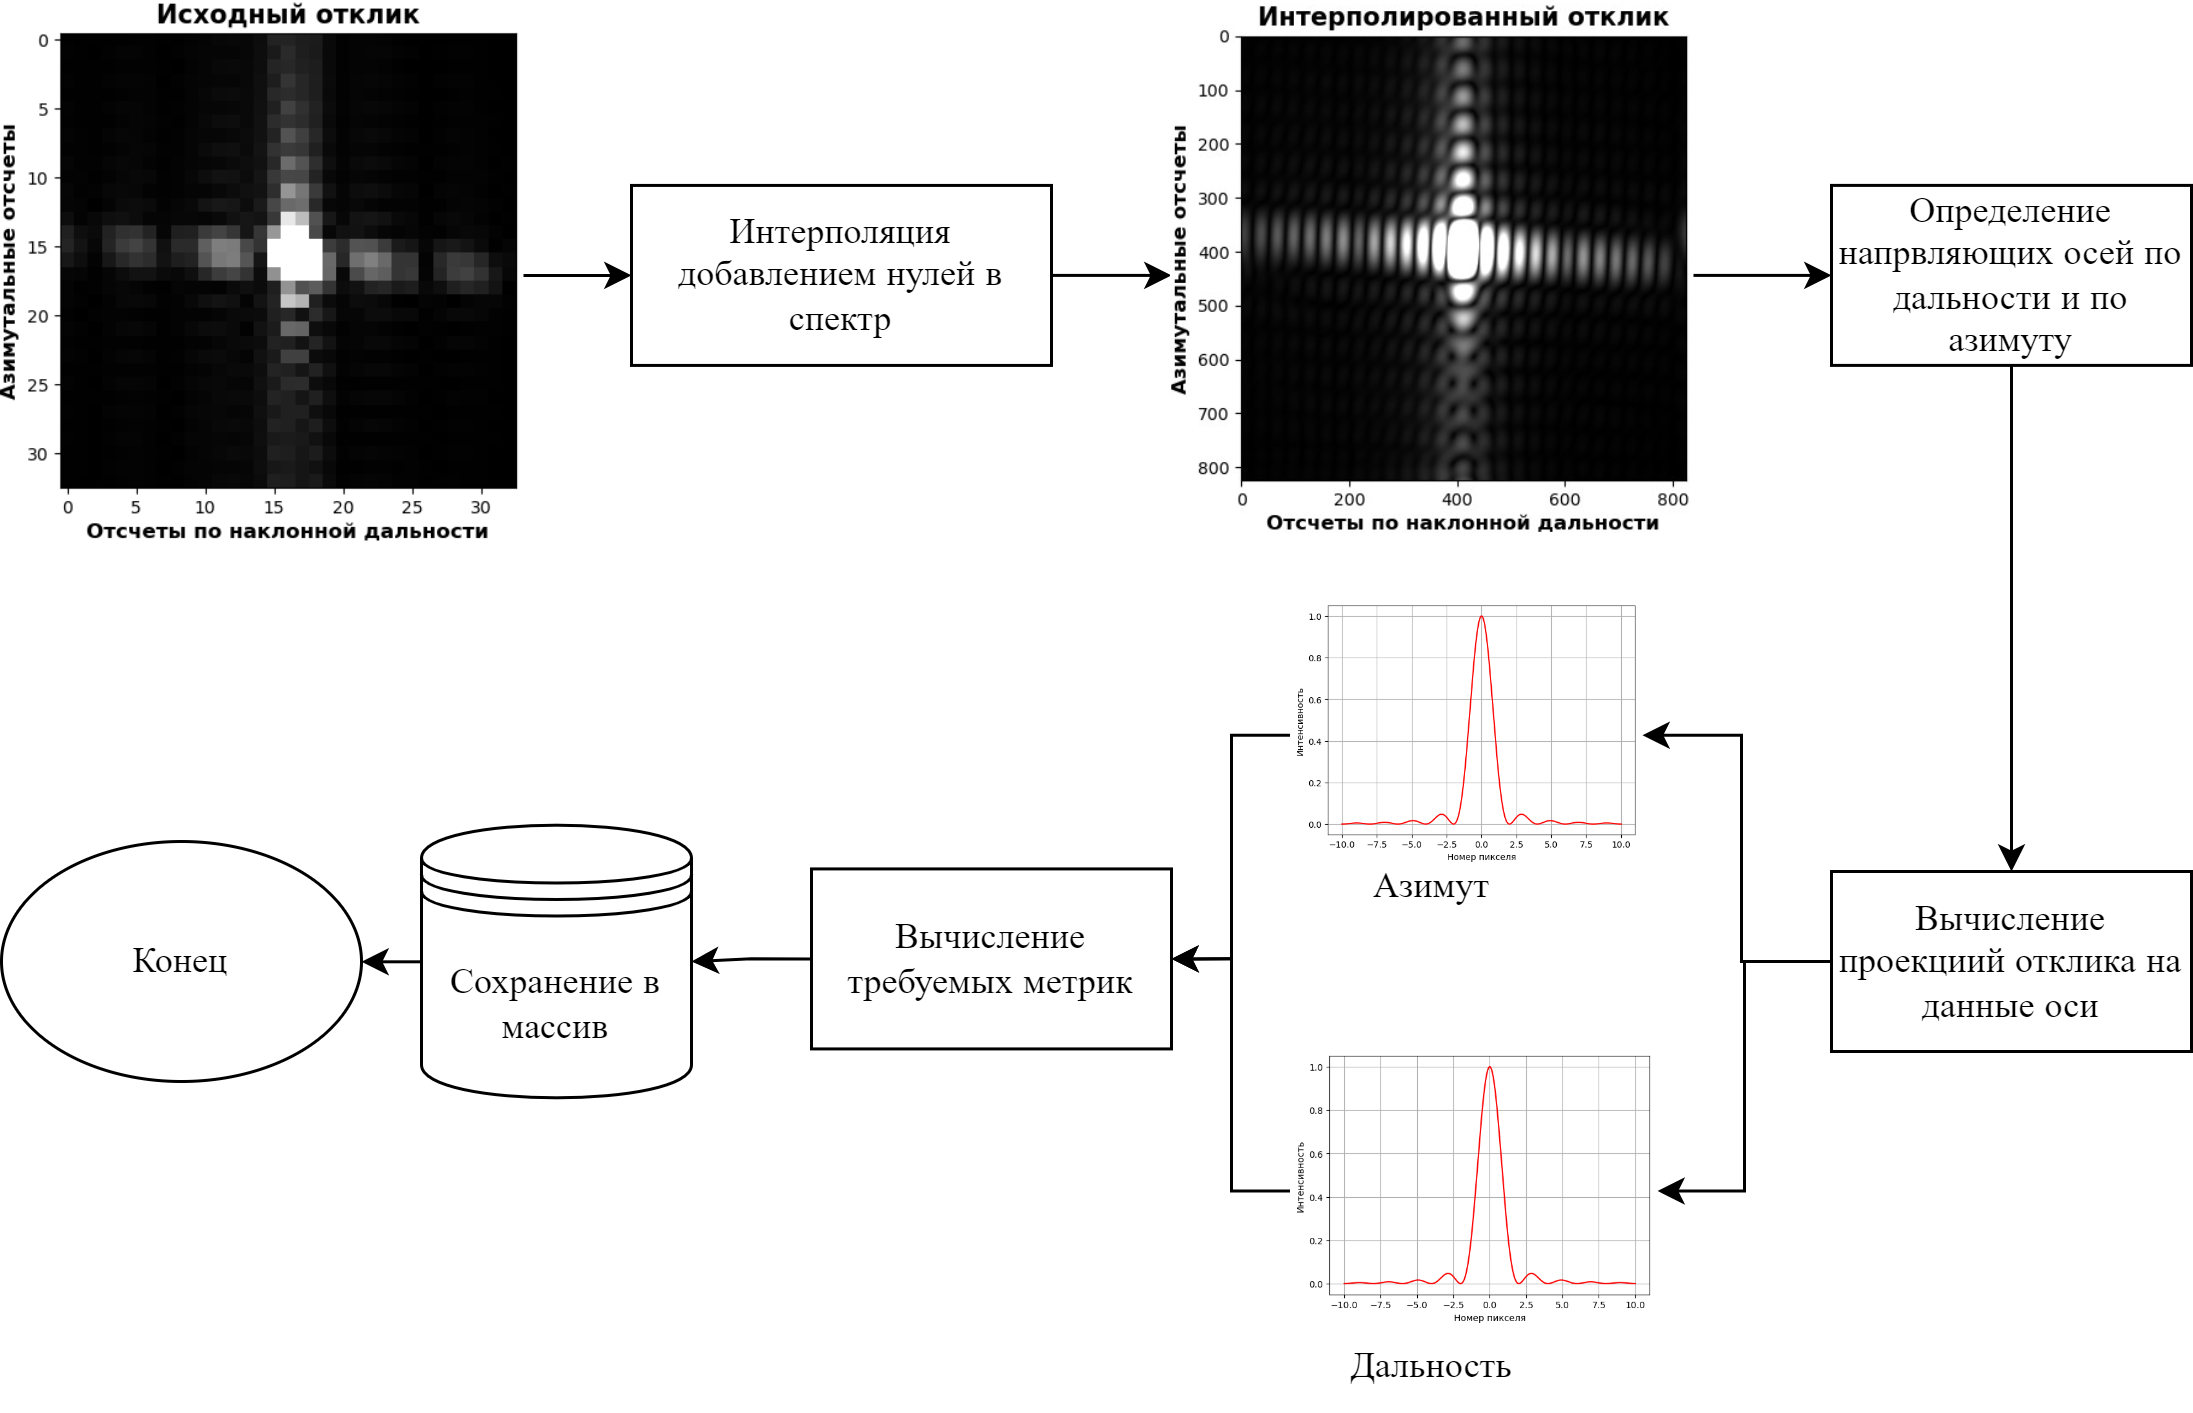
\includegraphics[width=1\textwidth]{alg_analys_targets.png}
    \caption{Алгоритм анализа псевдоточечных целей}
    \label{fig:alg_analys_targets}
\end{figure}

\section{Алгоритм автоматического поиска и анализа псевдоточечных целей}

	После объединения упомянутых выше алгоритмов и добавления статистического анализа распределений, итоговый алгоритм представлен на рисунке \ref{fig:alg}.

\begin{figure}[ht]
    \centering
    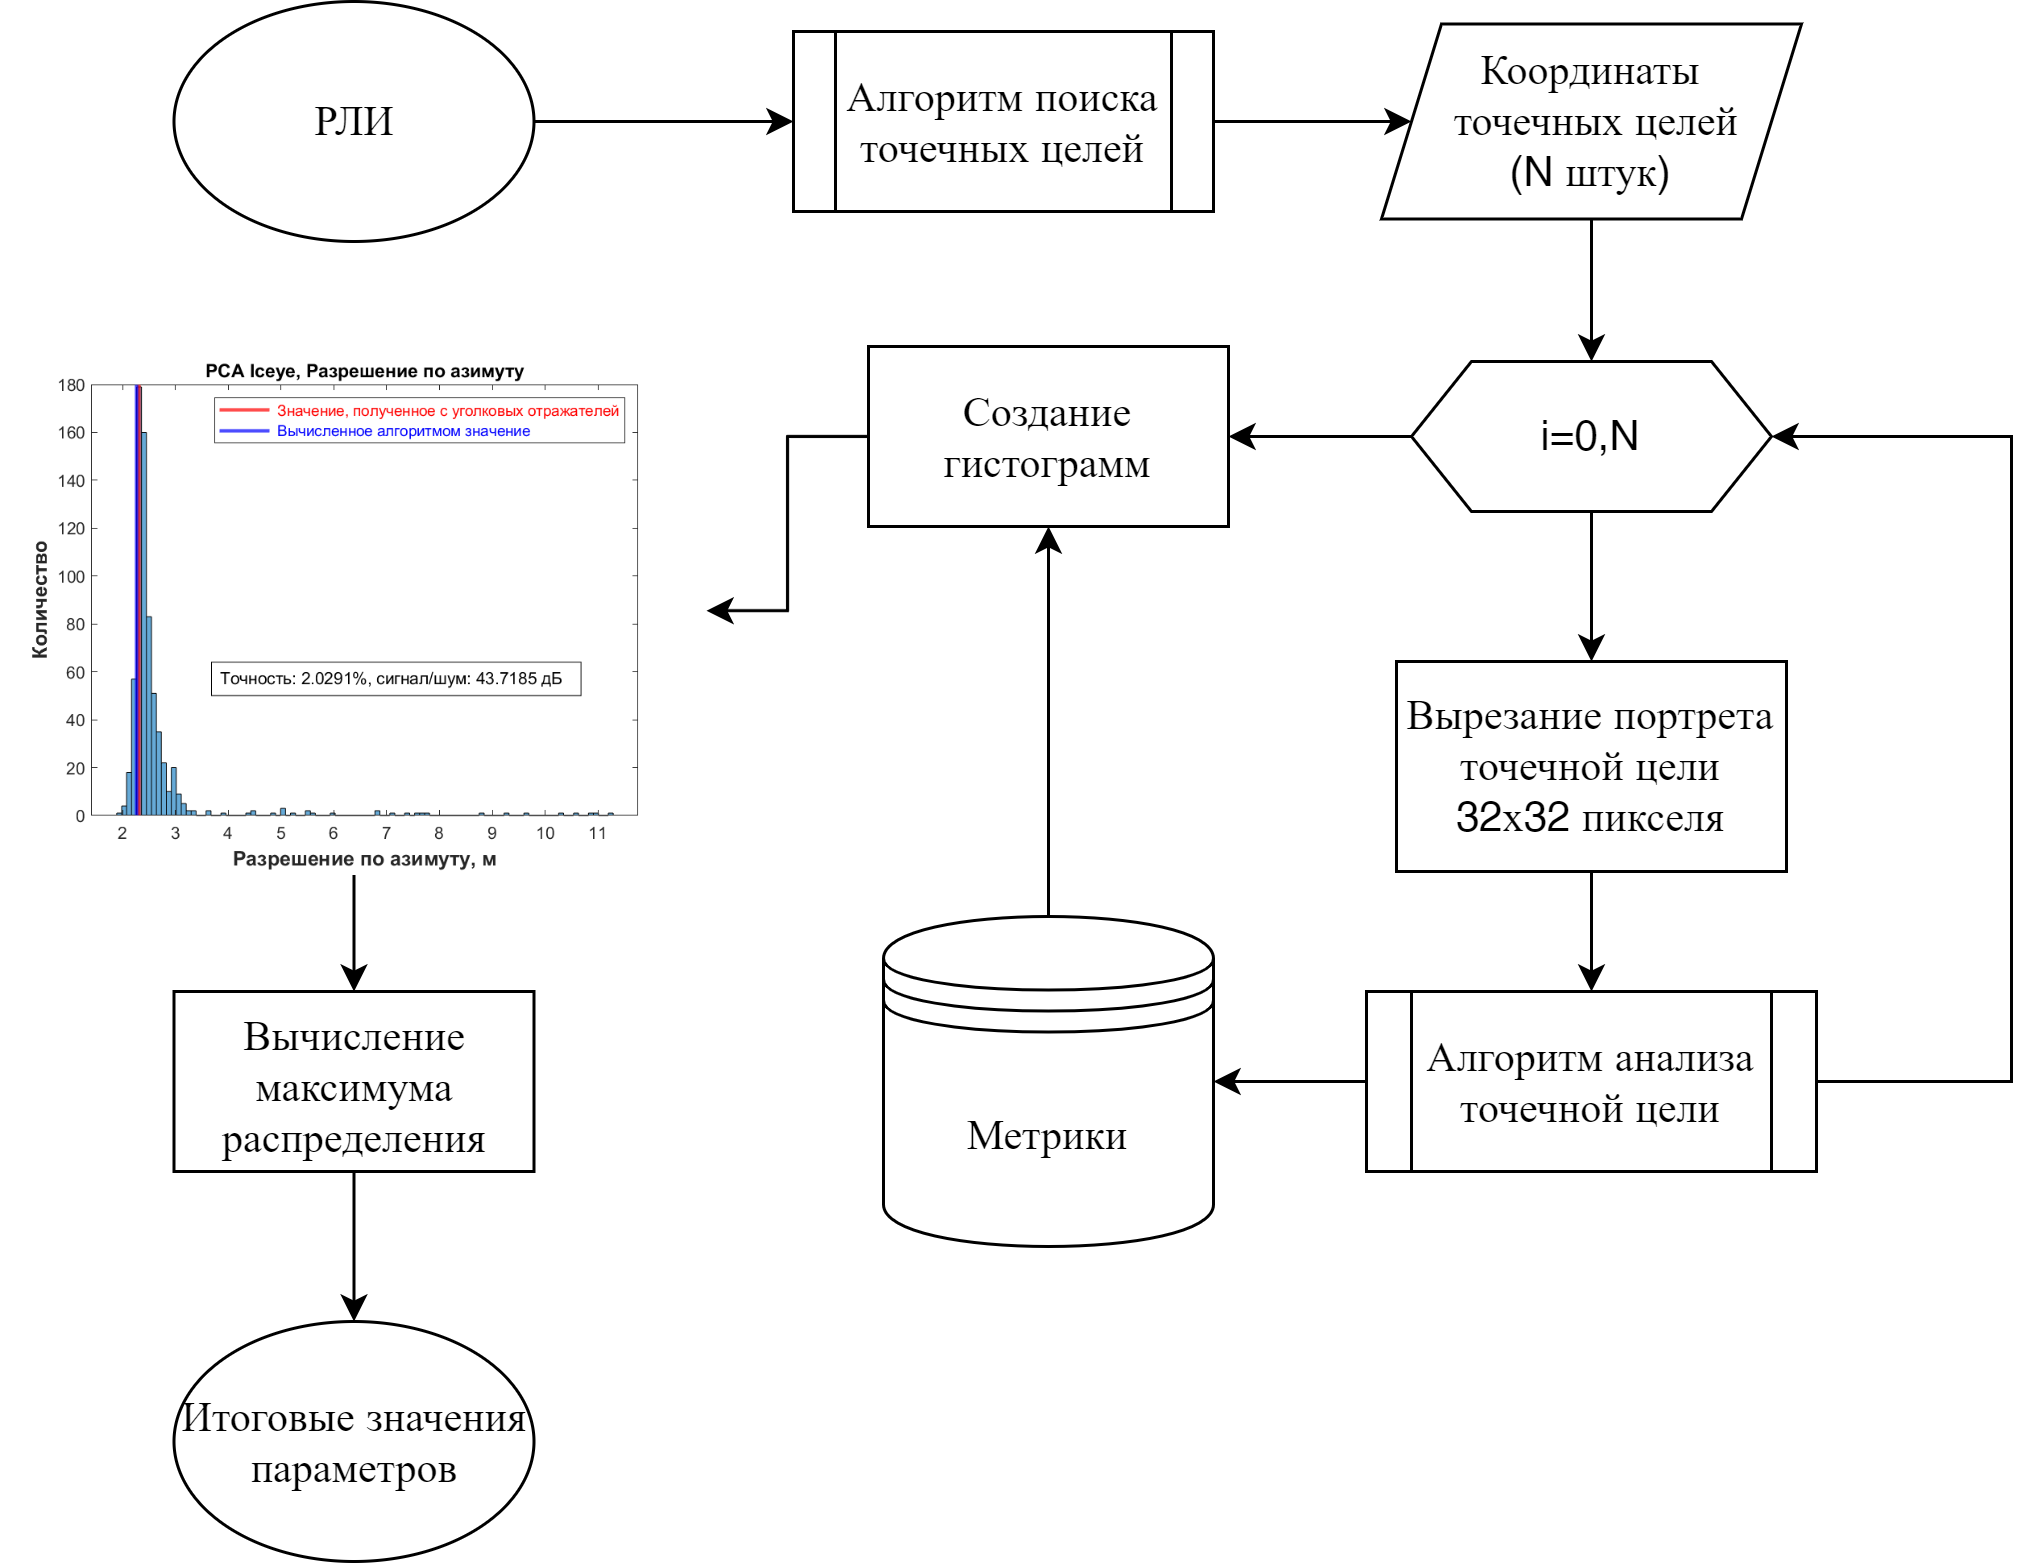
\includegraphics[width=1\textwidth]{alg.png}
    \caption{Алгоритм автоматического поиска и анализа псевдоточечных целей}
    \label{fig:alg}
\end{figure}

\newpage
 %% Исследование и построение решения задачи
    \chapter{Описание практической части}
\label{sec:Chapter4} \index{Chapter4}

	Алгоритм, описанный в предыдущей главе был реализован на языках Matlab и Python. В Matlab использовались  стандартные библиотеки, в Python - библиотеки numpy и scipy. 
	
\section{Калибровка алгоритма}

	Необходимым критерием для статистической оценке псевдоточечных целей является их наличие в диапозоне от 100 до 1000. Верхняя граница определяется возможностью вычислительных ресурсов ЭВМ. Для достижения поставленного критерия была выполнена калибровка алгоритма. Она заключается в установлении динамического порога при отборе псевдодочечных целей, который зависит от значения коэффициента эксцесса. Также был реализован динамический диапозон размеров клеток сетки, который зависит от размера входного изображения. Калибровка выполнялась на 22 радиолокационных снимков разного частотного диапазона.

\section{Верификация алгоритма}

	Для верификации работы алгоритма был выбран полигон с уголковыми отражателями Surat, который находится в Австралии. Полученные с уголковых отражателей значения разрешений сравнивались с результатом работы алгоритма. Соответствующие ошибки в определении разрешений представлены в таблице \ref{tab:errors}.
	
\begin{table}[]
    \centering
    \caption{Относительные ошибки в определении разрешений}
    \label{tab:errors}
    \begin{tabular}{|c|c|c|c|c|}
        \hline
        Название РСА  & Кол-во снимков  & Сигнал/шума, дБ  & $\epsilon$ & $\epsilon$  \\ \hline
        Iceye X-диапазон      & 7  & 43.9 & 1.09 & 1.80  \\ \hline
        Novasar-1 S-диапазон  & 11 & 38.7 & 0.73 & 3.11\\ \hline
        Sentinel-1 C-диапазон & 4  & 32   & 0.50 & 1.40  \\ \hline
        \multicolumn{3}{|c|}{Среднее значение} &  0.803 & 2.386 \\ \hline
    \end{tabular}
\end{table}

\section{Валидация алгоритма}

	В качестве валидации был обработан снимок Sentinel-1 в отсутсвии какой-либо информации о снимаемой сцене и, соответсвенно, в отсутвии уголковых отражателей. Результат обработки представлен на рисунке \ref{fig:senti}.
	
\begin{figure}[ht]
    \centering
    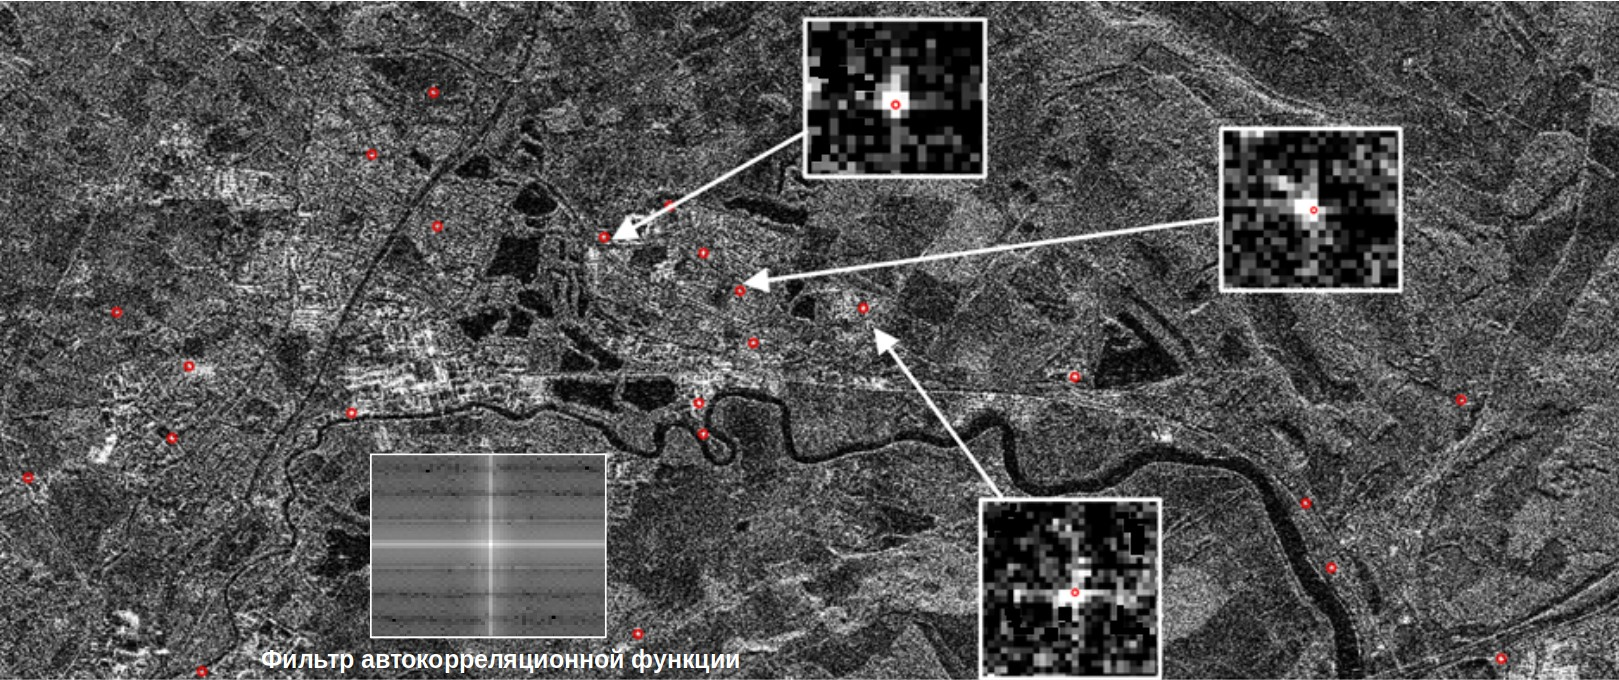
\includegraphics[width=1\textwidth]{senti.png}
    \caption{Снимок с РСА Sentinel}
    \label{fig:senti}
\end{figure}

	Полученные распределения и разрешения представлены на рисунке \ref{fig:distr}.	

\begin{figure}[ht]
    \centering
    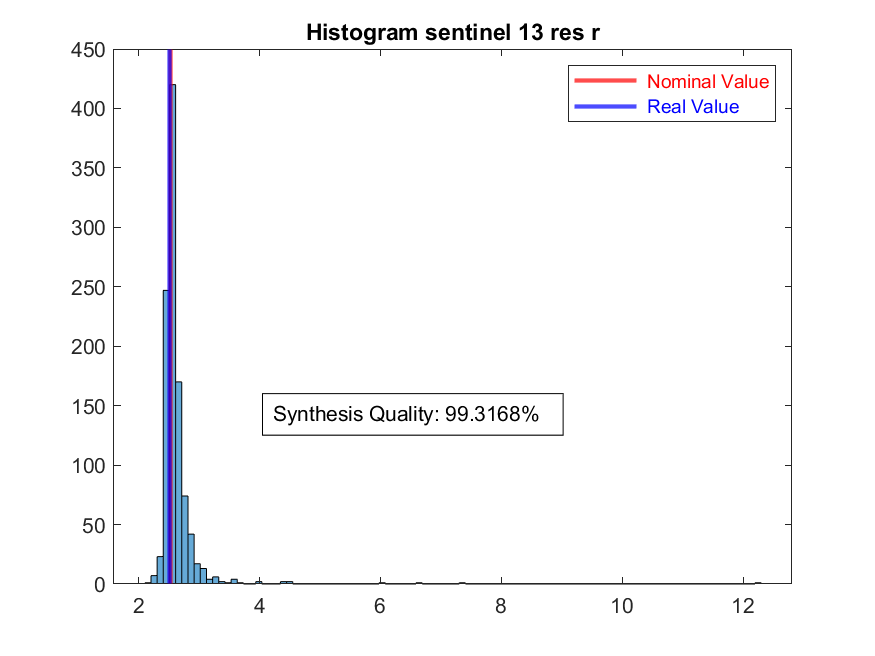
\includegraphics[width=1\textwidth]{distr.png}
    \caption{Гистограмма распределения разрешений}
    \label{fig:distr}
\end{figure}

	Полученные разрешения по дальности и по азимуту оказались равными 2.422 м 3.524 м соотвественно. При этом предельная разрешающая способность РСА равна 2.525 м и 3.56 м, что говорит о хорошем качестве синтеза изображения. То есть, коэффициент ухудшения равен соотвественно ... и ... .	

\newpage
 %% Описание практической части
    \chapter{Заключение}
\label{sec:Chapter5} \index{Chapter5}

	В данной работе был предложен метод определения качества синтеза РЛИ, основанный на анализе отклика от псевдоточечных целей. Представленная модель формирования отклика от псевдоточечных целей показала равенство между максимумом распределения разрешений псевдоточечных целей и разрешением точечной цели. Был разработан алгоритм поиска псевдоточечных целей на РЛИ, основанный на вычислении АКФ и коэффициента эксцесса. Также были разработаны алгоритмы анализа отклика от псевдоточечной цели и статистической оценке распределения разрешений. Разработанные алгоритмы были реализованы на языках Matlab и Python. Валидация разработанных алгоритмов была проведена на полигоне с уголковыми отражателями Surat (Австралия). Итоговая погрешность в определении разрешений по дальности и по азимуту составила 0.8\% и 2.37\% соответсвенно по дальности и по азимуту. Валидация на снимке Sentinel показала возможность работы со снимками без апприорной информации о снимаемой сцене. Исходя из постановки задачи исследования все требования были выполнены. 

	В дальнейшем планируется увеличить точность метода с помощью введения показателя точечности псевдоточечных целей и написание промышленного продукта для регулярного использования как в научных целей, так и в практических приложениях.

\newpage
 %% Заключение

    %% Don't change the following lines
    \nocite{*}
    \bibliography{references}

    %% в зависимости от надобности подключаем раздел "Приложениие"
    % \newpage
    % \section*{Приложение}
\addcontentsline{toc}{section}{Приложение}
\label{sec:Apendix} \index{Apendix}


\end{document}
